% Copyright (c) 2012 by Michał Nazarewicz <mina86@mina86.com>
% Distributed under the terms of the Creative Commons
% Attribution-ShareAlike 3.0 Unported (CC BY-SA 3.0) license.
\documentclass{beamer}
\usepackage[utf8]{inputenc}
\usepackage[T1]{fontenc}
\usepackage{lmodern}
\usepackage[english]{babel}
\usepackage{pgf}
\usepackage{units}
\usepackage{lmodern}
\usepackage{color}
\usepackage{listings}
\usepackage{amsmath}
\usepackage[super]{nth}

\newcommand{\notimplies}{%
  \mathrel{{\ooalign{\hidewidth$\not\phantom{=}$\hidewidth\cr$\implies$}}}}

% Define the Google colours.
\definecolor{GoogleBlue}{RGB}{51,105,232}
\definecolor{GoogleYellow}{RGB}{238,178,17}
\definecolor{GoogleGreen}{RGB}{0,153,37}
\definecolor{GoogleRed}{RGB}{213,15,37}
\newcommand\Google{\href{http://www.google.com/}{%
{\color{GoogleBlue}G}%
{\color{GoogleRed}o}%
{\color{GoogleYellow}o}%
{\color{GoogleBlue}g}%
{\color{GoogleGreen}l}%
{\color{GoogleRed}e}}}

\definecolor{gray}{RGB}{102,102,102}
\definecolor{darkgreen}{RGB}{0,128,0}

\lstset{
  language=C,
  basicstyle=\small\rmfamily,
  numbers=left,
  numberstyle=\tiny\color{gray},
  stepnumber=1,
  numbersep=5pt,
  showspaces=false,
  showstringspaces=false,
  showtabs=false,
  tabsize=8,
  captionpos=b,
  breaklines=true,
  breakautoindent,
  columns=fullflexible,
  morekeywords={inline,bool},
  keywordstyle=\color{blue}\bfseries,
  commentstyle=\color{darkgreen}\itshape,
  stringstyle=\color{red}\ttfamily
}
\lstdefinelanguage{diff}{
  morecomment=[f][\color{blue}]{@@},     % group identifier
  morecomment=[f][\color{red}]-,         % deleted lines
  morecomment=[f][\color{darkgreen}]+,   % added lines
  morecomment=[f][\color{gray}]{---},    % Diff header lines (must appear after +,-)
  morecomment=[f][\color{gray}]{+++},
}
\def\code{\lstinline[basicstyle=\rmfamily]}

\usetheme{Frankfurt}

% Shrink the margins slightly.
\setbeamersize{text margin left=5mm}
\setbeamersize{text margin right=5mm}

% Remove navigation symbols. They are never used anyway.
\setbeamertemplate{navigation symbols}{}

% Make more room on notes pages (when used).
\setbeamertemplate{note page}[plain]
\setbeamerfont{note page}{size=\scriptsize}

% gray footnotes, no rule.
% FIXME: This is broken. The gray continues onto subsequent slides.
% Note: footnotes are generally a bad idea in presentations.
\setbeamercolor{footnote mark}{fg=gray}
\renewcommand{\footnoterule}{}

\setbeamertemplate{footline}{}

\newcommand\Section[1]{%
\section{#1}%
\begin{frame}%
\frametitle{Outline}
\tableofcontents[currentsection]%,sections=\thesection]%
\end{frame}}


\newcommand\theauthor{Michał Nazarewicz}
\newcommand\theemail{mina86@mina86.com}
\title{Continuous Memory Allocator}
\subtitle{Allocating big chunks of physically contiguous memory}
\author[\theauthor]{%
  \texorpdfstring{\theauthor\vskip 8pt%
    \scriptsize\href{mailto:\theemail}{\theemail}}{%
    \theauthor}}
\institute{\Google}
\date{\today}

\setbeamerfont{institute}{size={\fontsize{10pt}{12pt}}}
\setbeamerfont{date}{size={\fontsize{8pt}{10pt}}}


\begin{document}

\begin{frame}
  \titlepage
\end{frame}

\begin{frame}
  \frametitle{Outline}
  \tableofcontents
\end{frame}

\Section{Introduction}
% Copyright (c) 2012 by Michał Nazarewicz <mina86@mina86.com>
% Distributed under the terms of the Creative Commons
% Attribution-ShareAlike 3.0 Unported (CC BY-SA 3.0) license.

\subsection{Why physically contiguous memory is needed}

\begin{frame}
  \frametitle{The mighty MMU}

  \begin{columns}[c]

    \column{.6\textwidth}
    \begin{itemize}
    \item Modern CPUs have MMU.
      \begin{itemize}
      \item Virtual $\rightarrow$ physical address.
      \end{itemize}
    \item Virtually contiguous $\notimplies$ physically contiguous.
    \item<1> So why bother?

    \item<2> MMU stands behind CPU.
    \item<2> There are other chips in the system.
    \item<2> Some require large buffers.
      \begin{itemize}
      \item<2> 5-megapixel camera anyone?
      \end{itemize}
    \item<2> On embedded, there's plenty of those.
    \end{itemize}

    \column{.4\textwidth}
    \begin{center}
      \includegraphics<1>[width=\textwidth]{build/mmu-iommu-images--img-mmu.eps}
      \includegraphics<2>[width=\textwidth]{build/mmu-iommu-images--img-nommu.eps}
    \end{center}

  \end{columns}
\end{frame}

\begin{frame}
  \frametitle{The mighty DMA}

  \begin{columns}[c]

    \column{.6\textwidth}
    \begin{itemize}
    \item DMA can do vectored I/O.
    \item Gathering buffer from scattered parts.
      \begin{itemize}
        \item {\footnotesize Hence also another name: DMA scatter-gather.}
      \end{itemize}
    \item Contiguous for the device $\notimplies$ physically contiguous.
    \item<1> So why bother?
    \item<2> DMA may lack vectored I/O~support.
    \item<2> DMA can do linear access only.
    \end{itemize}

    \column{.4\textwidth}
    \begin{center}
      \includegraphics[width=\textwidth]{build/mmu-iommu-images--img-dma.eps}
    \end{center}

  \end{columns}
\end{frame}

\begin{frame}
  \frametitle{The mighty I/O~MMU}

  \begin{columns}[c]

    \column{.6\textwidth}
    \begin{itemize}
    \item What about an I/O~MMU?
      \begin{itemize}
      \item Device $\rightarrow$ physical address.
      \end{itemize}
    \item Same deal as with CPU's MMU.
    \item<1> So why bother?
    \item<2> I/O~MMU is not so common.
    \item<2> I/O~MMU takes time.
    \item<2> I/O~MMU takes power.
    \end{itemize}

    \column{.4\textwidth}
    \begin{center}
      \includegraphics[width=\textwidth]{build/mmu-iommu-images--img-iommu.eps}
    \end{center}

  \end{columns}
\end{frame}

% Copyright (c) 2012 by Michał Nazarewicz <mina86@mina86.com>
% Distributed under the terms of the Creative Commons
% Attribution-ShareAlike 3.0 Unported (CC BY-SA 3.0) license.

\subsection{Solutions to the problem}

\begin{frame}
  \frametitle{Reserve and assign at boot time}

  \begin{itemize}
  \item Reserve memory during system boot time.
    \begin{itemize}
    \item \code{mem} parameter.
    \item Memblock / bootmem.
    \end{itemize}
  \item Assign buffers to each device that might need it.
  \item While device is not being used, memory is wasted.
  \end{itemize}
\end{frame}

\begin{frame}
  \frametitle{Reserve and allocate on demand}

  \begin{itemize}
  \item Reserve memory during system boot time.
  \item Provide API for allocating from that reserved pool.
  \item Less memory is reserved.
  \item But it's still wasted.
  \end{itemize}

  \begin{itemize}
  \item bigphysarea
  \item Physical Memory Manager
  \end{itemize}
\end{frame}

\begin{frame}
  \frametitle{Reserve but give back}

  \begin{itemize}
  \item Reserve memory during system boot time.
  \item Give it back
    \begin{itemize}
    \item but set it up so only movable pages can be allocated.
    \end{itemize}
  \item Provide API for allocating from that reserved pool.
  \item Migrate pages on allocation.
  \end{itemize}

  \begin{itemize}
  \item Contiguous Memory Allocator
  \end{itemize}
\end{frame}

\Section{Usage \& Integration}
\Section{Usage}{Using from device drivers}

\subsection{Overview}

\begin{frame}
  \frametitle{Overview}

  \begin{itemize}
  \item CMA is integrated with the DMA API.
  \item If device driver uses the DMA API, nothing needs to be changed.
  \item In fact, device driver should always use the DMA API and never
    call CMA directly.
  \end{itemize}
\end{frame}

\subsection{Allocating}

\begin{frame}[fragile]
  \frametitle{Allocating memory from device driver}

  \begin{block}{Allocation}
\begin{lstlisting}
void *my_dev_alloc_buffer(
    unsigned long size_in_bytes, dma_addr_t *dma_addrp)
{
    void *virt_addr = dma_alloc_coherent(
        my_dev, size_in_bytes, dma_addrp, GFP_KERNEL);
    if (!virt_addr)
        dev_err(my_dev, "Allocation failed.");
    return virt_addr;
}
\end{lstlisting}
  \end{block}

\end{frame}

\subsection{Releasing}

\begin{frame}[fragile]
  \frametitle{Releasing memory from device driver}

  \begin{block}{Freeing}
\begin{lstlisting}
void *my_dev_free_buffer(
    unsigned long size, void *virt, dma_addr_t dma)
{
    dma_free_coherent(my_dev, size, virt, dma);
}
\end{lstlisting}
  \end{block}
\end{frame}

\subsection{Integration with the architecture}

\begin{frame}
  \frametitle{Integration with the architecture}

  \begin{itemize}
  \item CMA needs to be integrated with the architecture.
  \item Memory needs to be reserved.
  \item There are early fixups to be done. {\footnotesize Or not.}
  \item The DMA API needs to be made aware of CMA.
  \item And Kconfig needs to be instructed to allow CMA.
  \end{itemize}
\end{frame}

\begin{frame}[fragile]
  \frametitle{Memory reservation}

  \begin{itemize}
  \item \code{memblock} must be ready, page allocator must not.
  \item On ARM, \code{arm_memblock_init()} is a~good place.
  \item All one needs to do, is call
    \code{dma_contiguous_reserve()}.
  \end{itemize}

  \begin{block}{Memory reservation}
\begin{lstlisting}
void __init dma_contiguous_reserve(
    phys_addr_t limit);
\end{lstlisting}
  \end{block}

  \begin{description}[limitAA]
  \item[{\ttfamily limit}] Upper limit of the region (or zero for no
    limit).
  \end{description}

\end{frame}

\begin{frame}[fragile]
  \frametitle{Memory reservation, cont.}

  \begin{block}{Reserving memory on ARM}
\begin{lstlisting}[language=diff]
 if (mdesc->reserve)
     mdesc->reserve();

+/*
+ * reserve memory for DMA contigouos allocations,
+ * must come from DMA area inside low memory
+ */
+dma_contiguous_reserve(min(arm_dma_limit, arm_lowmem_limit));
+
 arm_memblock_steal_permitted = false;
 memblock_allow_resize();
 memblock_dump_all();
\end{lstlisting}
  \end{block}
\end{frame}

\begin{frame}
  \frametitle{Early fixups}

  \begin{itemize}
  \item Kernel linear mapping uses huge pages.
  \item On ARM cache is not coherent.
  \item Having two mappings with different cache-ability gives
    undefined behaviour.
  \item So on ARM an “early fixup” is needed.
    \begin{itemize}
    \item This fixup alters the linear mapping so CMA regions use
      \unit[4]{KiB} pages.
    \end{itemize}
  \item The fixup is defined in
    \code{dma_contiguous_early_fixup()} function
    \begin{itemize}
    \item which architecture needs to provide
    \item with declaration in a~\code{asm/dma-contiguous.h} header file.
    \end{itemize}
  \end{itemize}
\end{frame}

\begin{frame}[fragile]
  \frametitle{Early fixups, cont.}

  \begin{block}{No need for early fixups}
\begin{lstlisting}
#ifndef ASM_DMA_CONTIGUOUS_H
#define ASM_DMA_CONTIGUOUS_H

#ifdef __KERNEL__

#include <linux/types.h>
#include <asm-generic/dma-contiguous.h>

static inline void
dma_contiguous_early_fixup(phys_addr_t base, unsigned long size)
{ /* nop, no need for early fixups */ }

#endif
#endif
\end{lstlisting}
  \end{block}
\end{frame}

\begin{frame}
  \frametitle{Integration with DMA API}

  \begin{itemize}
  \item The DMA API needs to be modified to use CMA.
  \item CMA most likely won't be the only one.
  \end{itemize}
\end{frame}

\begin{frame}[fragile]
  \frametitle{Integration with DMA API}

  \begin{block}{Allocate}
\begin{lstlisting}
struct page *dma_alloc_from_contiguous(
    struct device *dev,
    int count,
    unsigned int align);
\end{lstlisting}
  \end{block}

  \begin{description}[countAA]
  \item[{\ttfamily dev}] Device the allocation is performed on behalf
    of.
  \item[{\ttfamily count}] \emph{Number of pages} to
    allocate. {\footnotesize Not number of bytes nor order.}
  \item[{\ttfamily align}] Order which to align to.  Limited by
    Kconfig option.
  \item Returns page that is the first page of \code{count} allocated
    pages. {\footnotesize It's not a~compound page.}
  \end{description}
\end{frame}

\begin{frame}[fragile]
  \frametitle{Integration with DMA API}

  \begin{block}{Release}
\begin{lstlisting}
bool dma_release_from_contiguous(
    struct device *dev,
    struct page *pages,
    int count);
\end{lstlisting}
  \end{block}

  \begin{description}[countAA]
  \item[{\ttfamily dev}] Device the allocation was performed on behalf
    of.
  \item[{\ttfamily pages}] The first of allocated
    pages. {\footnotesize As returned on allocation.}
  \item[{\ttfamily count}] Number of allocated pages.
  \item Returns \code{true} if memory was freed (ie.\ was managed by
    CMA) or \code{false} otherwise.
  \end{description}
\end{frame}

\begin{frame}
  \frametitle{Let it compile!}

  \begin{itemize}
  \item There's one think that needs to be done in \code{Kconfig}.
  \item Architecture needs to \code{select HAVE_DMA_CONTIGUOUS}.
  \item Without it, CMA won't show up under “Generic Driver Options”.
  \item Architecture may also \code{select CMA} to force CMA in.
  \end{itemize}
\end{frame}

\subsection{Private \& not so private CMA regions}

\begin{frame}
  \frametitle{Default CMA region}

  \begin{itemize}
  \item Memory reserved for CMA is called CMA region or CMA context.
  \item There's one default context devices use.
  \item So why does \code{dma_alloc_from_contiguous()} take
    device as an argument?
  \item There may also be per-device or private contexts.
  \end{itemize}
\end{frame}

\begin{frame}
  \frametitle{What is a~private region for?}

  \begin{itemize}
  \item Separate a~device into its own pool.
    \begin{itemize}
    \item May help with fragmentation.
    \item For instance big vs small allocations.
    \item Several devices may be grouped together.
    \end{itemize}
  \item Use different contexts for different purposes within the same
    device.
    \begin{itemize}
    \item Simulating dual channel memory.
    \item Big and small allocations in the same device.
    \end{itemize}
  \end{itemize}
\end{frame}

\begin{frame}[fragile]
  \frametitle{Declaring private regions}

  \begin{block}{Declaring private regions}
\begin{lstlisting}
int dma_declare_contiguous(
    struct device *dev,
    unsigned long size,
    phys_addr_t base,
    phys_addr_t limit);
\end{lstlisting}
  \end{block}

  \begin{description}[countAA]
  \item[{\ttfamily dev}] Device that will use this region.
  \item[{\ttfamily size}] \emph{Size in bytes} to
    allocate. {\footnotesize Not pagas nor order.}
  \item[{\ttfamily base}] Base address of the region (or zero to use
    anywhere).
  \item[{\ttfamily limit}] Upper limit of the region (or zero for no
    limit).
  \item Returns zero on success, negative error code on failure.
  \end{description}
\end{frame}

\begin{frame}[fragile]
  \frametitle{Region shared by several devices}

  \begin{itemize}
  \item The API allows to assign a~region to a~single device.
  \item What if more than one device is to use the same region.
  \item It can be easily done via “copying” the context pointer.
  \end{itemize}
\end{frame}

\begin{frame}[fragile]
  \frametitle{Region shared by several devices, cont}

  \begin{block}{Copying CMA context pointer between two devices}
\begin{lstlisting}
static int __init foo_set_up_cma_areas(void) {
    struct cma *cma;
    cma = dev_get_cma_area(device1);
    dev_set_cma_area(device2, cma);
    return 0;
}
postcore_initcall(foo_set_up_cma_areas);
\end{lstlisting}
  \end{block}
\end{frame}

\begin{frame}
  \frametitle{Several regions used by the same device}

  \begin{itemize}
  \item CMA uses a~one-to-many mapping from \code{device} structure
    to CMA region.
  \item As such, one device can only use one CMA context\ldots
  \item \ldots unless it uses more than one \code{device}
    structure.
  \item That's exactly what S5PV110's MFC does.
  \end{itemize}
\end{frame}

\Section{Implementation}
% Copyright (c) 2012 by Michał Nazarewicz <mina86@mina86.com>
% Distributed under the terms of the Creative Commons
% Attribution-ShareAlike 3.0 Unported (CC BY-SA 3.0) license.

\subsection{Alokator stron}

\begin{frame}
  \frametitle{Algorytm bliźniaków}
  \begin{columns}[c]

    \column{0.6\textwidth}
    \begin{itemize}
    \item Alokator stron implementuje algorytm bliźniaków.
    \item Żądania w~kategoriach rzędu strony.
    \item Rząd może być 0--10\textcolor{gray}{$^\dagger$}.
    \item Zbyt duże strony są dzielone na połowy (tzw.\ bliźniaków).
    \item Podczas zwalniania, strona jest łączona z~bliźniakami.
    \end{itemize}

    \column{0.4\textwidth}
    \begin{center}
    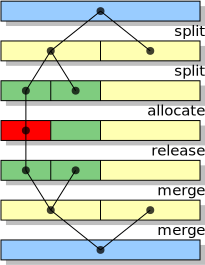
\includegraphics[width=0.9\textwidth]{build/alloc-free-cycle.eps}
    \end{center}
  \end{columns}
\end{frame}

\begin{frame}
  \frametitle{Strony i~bloki stron}
  \begin{center}
  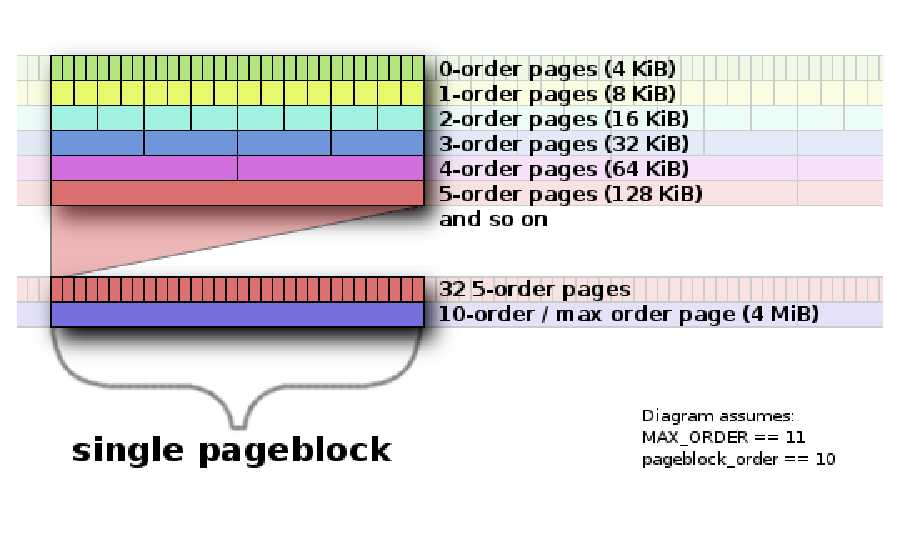
\includegraphics[width=0.9\textwidth]{build/pages.eps}
  \end{center}
\end{frame}

\begin{frame}[fragile]
  \frametitle{Typy migracji stron}

  \begin{itemize}
  \item Przy alokacji, użytkownik określa typ migracji żądanej strony:
    \begin{itemize}
    \item {\it unmovable}, {\it reclaimable} lub {\it movable},
    \end{itemize}
  \item Dla potrzeb CMA:
    \begin{itemize}
    \item {\it unmovable} i {\it reclaimable} $\rightarrow$ strony
      \textsl{nieruchome},
    \item {\it movable} $\rightarrow$ strony \textsl{ruchome}.
    \end{itemize}
  \end{itemize}
\end{frame}

\begin{frame}[fragile]
  \frametitle{Typy migracji bloków stron}

  \begin{itemize}
  \item Każdy blok stron ma przpisany typ migracji.
  \item Ułatwia to trzymanie stron tego samego typu razem.
  \item Przy alokacji strony są brane z~odpowiedniego bloku.
    \begin{itemize}
    \item Chyba, że takowych nie ma.
    \end{itemize}
  \item Typ bloku może się zmieniać.
  \end{itemize}
\end{frame}

\begin{frame}[fragile]
  \frametitle{Migracja}

  \begin{itemize}
  \item Strony ruchome, mogą być migrowane.
  \item Migracja polega na:
    \begin{itemize}
    \item skopiowaniu zawartości strony gdzie indziej i
    \item uaktualnieniu odwołań do starej strony.
    \end{itemize}
  \item Przykładami stron ruchomych są:
    \begin{itemize}
    \item anonimove strony procesów i
    \item bufory dyskowe.
    \end{itemize}
  \end{itemize}
\end{frame}

\subsection{CMA implementation}

\begin{frame}
  \frametitle{CMA implementation overview}

  \begin{itemize}
  \item CMA is build on the idea of migrating non-free pages.
  \item CMA needs guarantees that large number of contiguous pages can
    be migrated.
    \begin{itemize}
    \item 100\% guarantee is of course never possible.
    \end{itemize}
  \end{itemize}
\end{frame}

\begin{frame}[fragile]
  \frametitle{CMA migrate type}

  \begin{itemize}
  \item CMA had to introduce a~new migrate type.
    \begin{itemize}
    \item \lstinline|MIGRATE_CMA|
    \end{itemize}
  \item This migrate type has the following two important properties:
    \begin{itemize}
    \item CMA pageblocks never change migrate type.\footnote{Other
      than while CMA is allocating memory from them.}
    \item Only movable pages can be allocated from CMA pageblocks.
    \end{itemize}
  \end{itemize}
\end{frame}

\begin{frame}
  \frametitle{Preparing CMA region}

  \begin{itemize}
  \item At the boot time, some of the memory is reserved.
  \item When page allocator initialises, that memory is released with
    CMA's migrate type.
  \item This way, it can be used for movable pages.
    \begin{itemize}
    \item Unless the memory is allocated to a~device driver.
    \end{itemize}
  \item Each CMA region has a~bitmap of “CMA free” pages.
    \begin{itemize}
    \item “CMA free” page is one that is not allocated for device
      driver.
    \item It may still be allocated as a~movable page.
    \end{itemize}
  \end{itemize}
\end{frame}

\begin{frame}[fragile]
  \frametitle{Allocation}

  \begin{center}
    \includegraphics[width=\textwidth]{build/cma-alloc-algo.eps}
  \end{center}

\end{frame}

% Copyright (c) 2012 by Michał Nazarewicz <mina86@mina86.com>
% Distributed under the terms of the Creative Commons
% Attribution-ShareAlike 3.0 Unported (CC BY-SA 3.0) license.

\subsection{Podsumowanie}

\begin{frame}
  \frametitle{Problemy}

  \begin{itemize}
  \item Strony ruchome nie zawsze można zmigrować:
    \begin{itemize}
    \item \code{get_user_pages()}
    \item Strony dziennika ext4.
    \item Niektóre systemy plików.
    \end{itemize}
  \item Migracja zajmuje czas.
  \end{itemize}
\end{frame}

\begin{frame}
  \frametitle{Przyszłość?}
  \begin{itemize}
  \item Mądrzejszy dobór zakresu.
  \end{itemize}

  \begin{itemize}
  \item Stronicowanie.
  \item \href{http://code.google.com/p/compcache}{zRam}.
  \item \href{http://lwn.net/Articles/340080/}{Pamięć transcendentna}.
  \item \href{http://lwn.net/Articles/468896/}{\code{POSIX_FADV_VOLATILE}}.
  \end{itemize}
\end{frame}


\appendix

\section*{Q \& A}
\begin{frame}
  \begin{center}
    \vskip 2em
    {\Huge Thank you!}
    \vskip 2em
    
\includegraphics[width=0.3\textwidth]{build/interrogation.eps}
  \end{center}

  \vskip 2em

  \begin{itemize}
  \item \theauthor
  \item \href{mailto:\theemail}{\theemail}
  \item \url{http://mina86.com/cma/}
  \end{itemize}

  \vskip 1em
  \hfill \href{http://creativecommons.org/licenses/by-sa/3.0}{%
    \includegraphics[height=0.8em,clip=true]{build/cc-by-sa.eps}}
\end{frame}

\end{document}
